\title{Mastering the game of Connect 4 through self-play}
\author{
        Julian Wandhoven \\
                fgz\\
}
\date{\today}

\documentclass[12pt]{article}
\usepackage[dvipsnames]{xcolor}
\usepackage{amssymb}
\usepackage{tabularx}
\usepackage{titlesec}
\usepackage{amsmath}
\usepackage{svg}
\usepackage{caption}
\usepackage{hyperref}
\usepackage{lscape}
\usepackage{import}
\usepackage{caption}
\usepackage{subcaption}

\usepackage{rotating}
\usepackage{tikz}

\usepackage{graphicx}
\graphicspath{ {./images/} }

\setcounter{secnumdepth}{4}
\setcounter{tocdepth}{4}

\titleformat{\paragraph}
{\normalfont\normalsize\bfseries}{\theparagraph}{1em}{}
\titlespacing*{\paragraph}
{0pt}{3.25ex plus 1ex minus .2ex}{1.5ex plus .2ex}

\newcommand{\imgRef}[1]{(fig \ref{#1} on page \pageref{#1})}
\newcommand{\equationref}[1]{equation \ref{#1} on page \pageref{#1}}
\newcommand{\sectionref}[1]{section \ref{#1} on page \pageref{#1}}
\newcommand{\source}[1]{\caption*{Source: {#1}} }

\newcommand{\tickTackToe}[9]{
\begin{tabular}{p{7px}|p{7px}|p{7px}}
\multicolumn{3}{c}{}\\
  #1 & #2 & #3 \\      \hline
  #4 & #5 & #6 \\      \hline
   & #7 & #8\\
\multicolumn{3}{c}{#9}
\end{tabular}
}
\newcommand{\ticTacToe}[9]{
\begin{tabular}{p{7px}|p{7px}|p{7px}}
  #1 & #2 & #3 \\      \hline
  #4 & #5 & #6 \\      \hline
  #7 & #8 & #9 \\
\end{tabular}
}
\newcommand{\rewardArrow}[1]{\(\xrightarrow[\text{#1}]{\text{reward}}\) }

\newcommand{\FittedEloRaiting}{408}
\newcommand{\FittedScoringThreshold}{2.8}

\newcommand{\mathColor}[2]{\color{#1}#2\color{black}}
\newcommand{\gold}{YellowOrange}

\hypersetup{
    colorlinks=true,
    linkcolor=blue,
    filecolor=magenta,      
    urlcolor=blue,
    pdfpagemode=FullScreen,
    }

\urlstyle{same}

\begin{document}
\maketitle
\begin{abstract}
%\noindent A reimplementation of the Alpha Zero algorithm in C++ using the PyTorch library, based on the 2 papers by Google Deep Mind~\cite{silver2018general}\cite{silver2017mastering}.
\noindent Alpha Zero is an AI algorythem, that is capable of learning to play zero sum stated multiplayer games. These types of games include Go, Chess, Phi Sho and so forth. This is done by training a neural network and from data generated by a Monte Carlo Tree Serch. This document also explains how neural networks work and a short explenation of the infrastructure around the AI to allow for playing on remote devices.
~\cite{silver2018general}\cite{silver2017mastering}
\end{abstract}
%\newpage
\tableofcontents
\newpage

Alpha Zero is an algorithm published in 2018 by Google Deepmind as the generalization of AlphaGo Zero, an algorithm that learned to play the game of Go using only the rules of the game. In the generalized version, the same principles were applied to Chess and Shogi. Unlike previous algorithms such as StockFish or Elmo that use hand-crafted evaluation functions along with alpha-beta searches over a large search space, Alpha Zero uses no human knowledge. Rather, it generates all information through self-play. It has been shown to achieve superhuman performance in Chess, Shogi and Go. In this project the, AI will be trained to play connect4. The entire algorithm is implemented in C++ to increase efficiency during the Monte Carlo Tree Search (MCTS). Furthermore, to allow for better performance when playing, all computations are handled via a server (my desktop). A secondary server has also been added to allow for easy re-routing of the main server and handle things like elo-ratings (see \sectionref{sec:Evaluation:elo-rating}) for all agents. Additionally, I have added a short introduction on how neural networks work and how they are trained in \sectionref{NN}. 

\section{Methods}
\label{Methods}
The Alpha Zero algorithm is a reinforcement learning algorithm using two major parts: a) a {\it Monte Carlo tree search} (MCTS) that is guided by b) the {\it neural network} to improve performance. \\\\
The agent (computer player) runs a certain amount of simulation games using its MCTS and neural network. At each step, the MCTS evaluates the most promising next states as given by the neural network's estimation. The MCTS, by simulating games starting from the current state, will improve the neural network's prediction for that state. At the end of each game, the winner is determined and used to update the neural network's estimation of who would win a game starting from a certain state.
\subsection{Reinforcement Learning}
When training neural networks, there are three major possible situations: Supervised learning, unsupervised learning, and reinforcement learning. The first uses predetermined data with known in- and outputs the network is trained to predict. An example of supervised learning is the recognition of handwriting as the data is defined by humans. This method consists of creating a large database of examples, and the neural network is then trained to predict a given output for all examples. 

Unsupervised learning or self-organization is used when there is no previous available data and the neural network has to create those classifications itself. An example of unsupervised learning is image generation (DCGAN (Deep Constitutional Generative Adversarial neural networks)) as the output of the network is not defined by the programmer and the input is random noise. Image generation consists of two networks. The first network \(\theta_g\) is used to generate images. The second network \(\theta_c\) is the critic network used to evaluate how good  \(\theta_g\) is. The algorithm consists of generating images with \(\theta_g\) and using  \(\theta_c\) to try and distinguish them from some example outputs.

These two methods represent the extreme ends of the spectrum. Reinforcement leaning on the other hand can be thought of as an intermediate form. It uses a predetermined environment which gives positive, neutral and negative feedback. The neural network is then discouraged from taking actions leading to negative feedback and encouraged to take actions leading to positive feedback. The feedback is determined by the environment the agent learns to interact with. In this case, losing a game would be bad and result in negative feedback whereas winning a game leads to positive feedback. Ties lead to neutral feedback. The agents learning is set up in such a way, that it is encouraged to take actions leading to positive feedback and discouraged from taking actions that lead to negative feedback. However actions, can lead to a loss that only occurs many game steps in the future. A common approach to solve this problem is to have the feedback propagate backwards to previous actions. In Alpha Zero, this is handled by the memory (see \sectionref{sec:memory}). When the game reaches an end state and a winner is determined, the feedback is propagated backwards up the game. If the player won, the feedback is positive. If he lost, it is negative. More specifically, if a player takes an action \(a\) at a state \(s\), that leads to a win, the reward for that state is defined as \(R(s,a) = 1\). On the other hand, if the action leads to a loss, the reward will be \(R(s, a) = -1\). If the game ends in a tie, the reward is \(R(s,a) = 0\). Every agent \(p\) will try to maximize \(\sum_{s\in g\cap p} R(s, a)\). \(g\cap p\) is the set of all states in which the player \(p\) takes an action. Let's look at a tic tac toe example of the following game:
\begin{center}
\tickTackToe{}{}{}{}{}{}{}{}{player X} \to \tickTackToe{X}{}{}{}{}{}{}{}{player O} \to \tickTackToe{X}{O}{}{}{}{}{}{}{player X} \to \tickTackToe{X}{O}{}{}{X}{}{}{}{player O} \to \tickTackToe{X}{O}{}{O}{X}{}{}{}{player X} \to \tickTackToe{X}{O}{}{O}{X}{}{}{X}{}
\end{center}
Since player \(X\) won the game, the reward for every state \(s\in g\cap X\) is \(R(s, a) = 1\) and the reward for every state \(s\in g\cap O\) is \(R(s, a) = -1\). The reward for the entire game is:
\begin{center}
\tickTackToe{}{}{}{}{}{}{}{}{} \rewardArrow{1} \tickTackToe{X}{}{}{}{}{}{}{}{} \rewardArrow{-1} \tickTackToe{X}{O}{}{}{}{}{}{}{} \rewardArrow{1} \tickTackToe{X}{O}{}{}{X}{}{}{}{} \rewardArrow{-1} \tickTackToe{X}{O}{}{O}{X}{}{}{}{} \rewardArrow{1} \tickTackToe{X}{O}{}{O}{X}{}{}{X}{}
\end{center}

The important thing to keep in mind is that reinforcement learning algorithms encourage actions that lead to a positive feedback and discourage actions that lead to a negative feedback.
\subsection{Game}
The game is the environment, that is used to train the AI by simulating it in the MCTS. The game consists of constant unchanging game states. Every game state consists of a game board and a player. An end game state is a state at which the game is done. This means that one player won or the game ended in a tie. For connect4 this means four stones in a line or a full game board.
Let \(\mathbb{G}\) be the set of all legal game states.
Let \(\mathbb{G}_{done}\) be the set of all game states for which the game is done. 
\subsubsection{Game Board}
Board games consist of placing stones of different types on a board with a certain amount of fields. Many games, like Go, Chess and Connect4, arrange their fields in a rectangular pattern. These games have two distinct stones. We can represent these game boards as stack of binary layers. Every layer is associated with one kind of stone. Each layer contains a one, where the board has a stone of the appropriate type and zeros everywhere else. For instance, the following tic tac toe game board can be represented by the following binary plane stack.\[
\ticTacToe{}{X}{O}{O}{X}{}{O}{}{X}\to
\left[ 
\begin{bmatrix}
0 & 1 & 0 \\
0 & 1 & 0 \\
0 & 0 & 1 \\
\end{bmatrix}
\begin{bmatrix}
0 & 0 & 1 \\
1 & 0 & 0 \\
1 & 0 & 0 \\
\end{bmatrix}
\right]
\] 
Internally, the game board is represented by a flat vector. The conversion from a game state \(s \in \mathbb{G}\) to a vector is identical to the numpy.flatten function. The flattening function is referred to as \(\left<s\right>_f\) and is defined as:
\[
\left<
\left[ 
\begin{bmatrix}
a_{111} & \cdots & a_{11o} \\
\vdots & \ddots & \vdots \\
a_{1n1} & \cdots & a_{1no} \\
\end{bmatrix}
\cdots
\begin{bmatrix}
a_{m11} & \cdots &  a_{m1o} \\
\vdots   & \ddots & \vdots   \\
a_{mn1} & \cdots & a_{mno}  \\
\end{bmatrix}
\right]
\right>_f = \begin{matrix}
[ a_{111} & a_{112} & \cdots &  a_{11o} \\
\cdots & a_{1n1}  & \cdots & a_{1no} \\
 a_{m11}  & \cdots & a_{m1o} & \cdots    \\
  a_{mn1} & \cdots   & a_{mno}]\\
\end{matrix}
\]
This operation for the tic tac toe board from before would look like this:
\[
\left<\ticTacToe{}{X}{O}{O}{X}{}{O}{}{X}\right>_f = 
[0\,1\,0\,0\,1\,0\,0\,0\,1\,0 \,0 \,1\,1\,0\,0\,1\,0\,0]
\]
\subsubsection{Actions}
Actions are numbers used to identify changes to the game. Every game has a set of all possible actions \(\mathbb{A}_{possible} \subset \mathbb{N}_0\). In connect4, the set of all possible actions is \(\mathbb{A}_{possible} = [0, 41]\). Every number is associated with a position on the game board. The mapping \(a\) to game fields is the following:
\begin{center}
\begin{tabular}{| c | c | c | c | c | c | c |}
 \hline
0 & 1 & 2 & 3 & 4 & 5 & 6  \\\hline
7 & 8 & 9 & 10 & 11 & 12 & 13\\\hline
14 & 15 & 16 & 17 & 18 & 19 & 20 \\\hline
21 & 22 & 23& 24 & 25 & 26 & 27 \\\hline
28 & 29 & 30 & 31 & 32 & 33 & 34 \\\hline
35 & 36 & 37 & 38 & 39 & 40 & 41 \\\hline
\end{tabular}
\end{center}
Let \(\mathbb{A}(s)\) be the set of all legal actions for a given state  \(s \in \mathbb{G}\). For all states \(s_{done} \in \mathbb{G}_{done}\) the set of all legal actions \(\mathbb{A}(s_{done})\) is the empty set. The function \(\mathcal{A}~:~\mathbb{G}, \mathbb{A}\to\mathbb{G}\) is used to get from one game state to another by taking an action.

\subsection{MCTS}
A Monte Carlo tree search (MCTS) is a tree search algorithm that can be used to find sequences of actions leading to a desirable outcome. This is done by procedurally generating a directed graph of possible successor states to the current state or root state. 

This graph consists of nodes that are used to simulate possible sequences of states starting from a root state and edges that connect nodes. The set of all possible nodes \(\mathbb{M}_{possible} = \{\mathcal{N}(s)~|~ s \in \mathbb{G}\}\), where \(\mathcal{N}:\mathbb{G}\to\mathbb{M}_{possible}\) is a bijective function that maps a game state to a node. \(\mathcal{S}~:~\mathbb{M}_{possible}\to\mathbb{G} = \mathcal{N}^{-1}\) is the inverse of \(\mathcal{N}\). The set of all allowed actions for a certain node \(n\in\mathbb{M}_{possible}\) is \(\mathbb{A}(n) = \mathbb{A}(\mathcal{S}(n))\) . The set of all nodes in an MCTS at any given time is \(\mathbb{M} \subseteq \mathbb{M}_{possible}\). Every node \(n \in \mathbb{M}\) has a set of edges \(\mathbb{E}(n)\) that connect it to other nodes, the set of all possible edges is \(\mathbb{E}_{possible}\). \(\mathcal{E}:~\mathbb{M}, \mathbb{A}_{possible} \to \mathbb{E}_{possible}\) is a bijective function used to map nodes and actions to edges. Furthermore for \(\mathcal{E}(n, a)\) to be valid \(a\) must be an element of \(\mathbb{A}(n)\).  The function \(\mathcal{N}_{to}~:~\mathbb{E}\to\mathbb{M}\) maps an edge to the node it is pointing to while \(\mathcal{N}_{from}~:~\mathbb{E}\to\mathbb{M}\) is used to find the node an edge is pointing from.
There are, however, two different kinds of nodes, that can be distinguished by the set of their edges. The first are the expanded nodes \(\mathbb{M}_{expanded}\subseteq\mathbb{M}\). For expanded nodes \( n\in \mathbb{M}_{expanded}\) the set of edges \(\mathbb{E}(n) = \{\mathcal{E}(n,a)~|~ a\in \mathbb{A}(n)\} \neq \emptyset\). The second category are the leaf nodes \(\mathbb{M}_{leaf} \subseteq \mathbb{M}\). Leaf nodes are unexpanded nodes. This means that they do not yet have any connections to other nodes. Thus \(\mathbb{E}(n) = \emptyset\) for all \(n \in \mathbb{M}_{leaf}\).

MCTS simulations consist of four phases: selection, evaluation, expansion, and back propagation. Every simulation starts from the MCTS's root node \(n_0 \in \mathbb{M}\). The selection phase of the MCTS is used to select a leaf node \(n_L \in \mathbb{M}_{leaf}\). This is done by using a selection function \(\sigma~:~\mathbb{M}\to\mathbb{M}\). This function is used to find node \(n_{t+1}\) from node \(n_t\) for \(t\in [0,L[\). \(n_{t+1}\) is selected by \(\sigma\).
\begin{equation}
\sigma(n_t) = n_{t+1}
\end{equation}
 This means that \(n_1 = \sigma(n_0)\), \(n_2 =  \sigma(n_1)\) \dots. When a leaf node is found, that leaf node is evaluated. In Alpha Zero this is achieved using the neural network described in section \ref{NN}. The neural network evaluates the leaf node using its evaluation function \(\theta~:~\mathbb{M}\to \mathbb{R},~\mathbb{R}^{|\mathbb{A}_{possible}|}\). The neural network's first output is an estimation of the expected reward. The expected reward can be thought of as the probability of winning minus the probability of loosing games starting at \(n_L\). The neural network's second output is the action policy \(p\in\mathbb{R}^{|\mathbb{A}_{possible}|}\) that represents the advantagiousness of the actions in \(\mathbb{A}_{possible}\). \(n_L\) is now expanded. Expansion works by creating nodes \(\mathbb{M}_{new} = \{\mathcal{N}(\mathcal{A}(\mathcal{S}(n_L), a)) | a \in \mathbb{A}(n_L)\}\) unless these nodes already exist. These new nodes are added to the MCTS. Furthermore, \(n_L\)'s edges are redefined as \(\mathbb{E}(n_L) = \{\mathcal{E}(n_L, a) | a \in \mathbb{A}(n_L)\}\). By definition \(\mathcal{N}_{to}(\mathcal{E}(n_L, a) = \mathcal{N}(\mathcal{A}(\mathcal{S}(n_L), a))\) for \(a\in\mathbb{A}(n_L)\). This can lead to \(n_L\) being moved from \(\mathbb{M}_{leaf}\) to \(\mathbb{M}_{expanded}\). During back propagation the expected reward of \(n_L\) is used to update the expected reward of all nodes traversed during selection. This effectively improves the estimation of the expected reward. This four step simulation is carried out a certain amount of times. The estimation error for all estimations of the expected reward will converge to \(0\) as the amount of simulations increases. The advantageousness of all actions \(a  \in \mathbb{A}(n_0)\) will also be given by the expected rewards of all successor states to \(n_0\). \imgRef{MCTS-simulation}

\subsubsection{Evaluation Basis}
The MCTS's goal is to find good estimations of the reward for a certain action at a certain state. This reward estimation is \(Q~:~\mathbb{E}_{possible}\to \mathbb{R}\). To define \(Q\), the functions \(W~:~\mathbb{E}\to\mathbb{R}\) and \(N~:~\mathbb{E}\to\mathbb{N}_0\) are required. \(N(e)\) is the amount of times an edge \(e\in\mathbb{E}_{possible}\) has been traversed. This means how many times \(\sigma\) has chosen to follow the edge \(e\) to a new node. \(W(e)\) is the sum of the reward computations from all \(N(e)\) times the edge has been evaluated. Therefore the expected reward \(Q\) is defined as:
\begin{equation}
Q(e) = \frac{W(e)}{N(e)}
\end{equation}
The fourth and last of these functions is \(P~:~\mathbb{E}\to\mathbb{R}\). \(P\) is the policy function, it's the neural network's preliminary estimation of \(P(e) \approx \frac{N(e)}{\sum_{i\in\mathbb{E}(\mathcal{N}_{from}(e))}N(i)}\). This function is used to guide the search to more promising edges before a lot of time is spent on simulation.

\subsubsection{Leaf Selection} \label{sec:Methods:MCTS:Leaf_selection}
MCTS's evaluation starts by simulating future moves within the tree. This is done by selecting an edge and then following that edge to a new node. From there, the next edge and node are selected. This is repeated until a leaf node is reached. To select an edge and thus a node from the current node \(n\in \mathbb{M}\) the function \(\sigma\) is used. To define \(\sigma\) we must first define the edge evaluation function \(v~:~\mathbb{E}\to\mathbb{R}\). \(v\) is defined as follows:
\begin{equation}
v(e) = Q(e) + c_{puct}P(e)\cdot\frac{\sqrt{\Sigma_{b\in\mathbb{E}(\mathcal{N}_{from}(e))}N(b)}}{1+N(e)}
\end{equation}
Where \(c_{puct}\in \mathbb{R}^+\) is the exploration constant used to define how important exploration is. The smaller \(c_{puct}\) is, more important \(Q\) and less important exploration and \(P\). \(\sigma\), for a given node \(n\in\mathbb{M}\), is then defined as:
\begin{equation}
\sigma(n) = \mathcal{N}_{to}(\text{argmax}(\mathbb{E}(n)))
\end{equation}
argmax returns the edge \(e\) with the largest \(v(e)\).
\(\sigma\) is run, until its output is a leaf-node \(N_L\in\mathbb{M}_{leaf}\).

\subsubsection{Node Evaluation and Expansion}
When a leaf node \(n_L\in\mathbb{M}_{leaf}\) is reached, that is not an end game node \(\mathcal{S}(n_L)\not\in\mathbb{G}_{done}\), the node is passed to the neural network. The neural network (see section \ref{NN}) is used to predict the node's policy \(p\) and its value \(v\). \(\theta(n_L) = (v, p)\). \(p\) is used to create new nodes \(\mathbb{M}_{new} = \left\{\mathcal{N}(\mathcal{A}(\mathcal{S}(n_L), a))~:~a\in\mathbb{A}(n_L)\right\}\). The initial function outputs of the three edge functions for the edges \(e\in\mathbb{E}(n_L)\), connecting \(n_L\) to \(\mathbb{M}_{new}\), are.
\[
N(e) = 0
\]
\[
W(e) = 0
\]
\[
P(e) = \pi(e)
\]
\(\pi(e)\) is the of the policy of the edge. It's defined as:
\[
\pi(\mathcal{E}(n_L, a)) = p_{a+1}
\]
where \(a\) is the edges action \(a \in \mathbb{A}(n_L)\). \(\mathbb{M}_{new}\) is then added to \(\mathbb{M}\).

\subsubsection{Backfill}
The value \(v\) is used to update the reward prediction for all nodes \(n_{[0, L]}\) traversed during the edge selection. Assuming that \(\rho~:~\mathbb{E}_{possible}\to\{1,\,-1\}\) is the player taking an action at an edge \(e\in\mathbb{E}_{possible}\), \(W\) and \(N\) are updated as follows for all nodes \(n_t\) with \(t\in [0,L]\):
\begin{align*}
N(n_t) + 1 &\Rightarrow N(n_t)\\
W(n_t) + v \cdot \rho(n_t) \cdot \rho(n_L) &\Rightarrow W(n_t)\\
\end{align*}

%-------------------------------------------------------------------------
\subsection{Neural Network}
Search algorithms like MCTS are able to find advantageous action sequences. In game engines, the search algorithm is improved by using evaluation functions. These functions are generally created using human master knowledge. In the Alpha Zero algorithm, this evaluation function is a biheaded deep convolutional neural network trained by information gathered from the MCTS. In order to understand the training process, one must first understand how the neural network functions.
\label{NN}
\subsubsection{Introduction to Neural Networks}
An artificial neural network or just neural network is a mathematical function inspired by biological brains. Although there are many types of neural networks, the only relevant one to this work is the feed forward network. These models consist of multiple linear computational layers separated by non-linear activation functions. Every layer takes the outputs of the previous layer, and applies a linear transformation to it~\cite{zhang2018artificial}. There are many different feed-forward neural network layers and activation functions to chose from when designing a neural network. To focus this explanation, only the relevant ones will be discussed along with the back-propagation algorithm.
\paragraph{Fully Connected Layer}
A fully connected layer is the most basic layer. It applies a simple matrix multiplication. The layer takes a \(1 \times n\) dimentional matrix \(x \in \mathbb{R}^{1\times n}\) as an input and multiplies it by a weight matrix \(w \in\mathbb{R}^{n\times m}\). This operation outputs a \(1\times m\) dimensional matrix to which a bias \(b \in \mathbb{R}^{1 \times m}\) is added to form the output matrix \(v \in \mathbb{R}^{1 \times m}\) containing the output values of the layer. \(v\) is then fed to the next layer. The addition of the bias vector \(b\) is optional. In some situations it is worth dropping the bias in favour of computational speed. The fully connected layer forward propagation function shall be defined as \(\delta_{wb}~:~\mathbb{R}^n\to\mathbb{R}^m\)
\begin{equation} \label{eq:NN:fully_connected_layer_forward}
\delta_{wb}(x) = w \cdot x + b
\end{equation}
\paragraph{Convolutional Layer}
Convolutional layers are commonly used for image processing. They perform the same operations over the entire image searching for certain patterns. In order to achieve this, a set of kernels \(\mathbb{K}\), of size \(m\times n\), are defined for the layer. Kernels are similar to fully connected layers. They consist of a weight tensor \(w\in\mathbb{R}^{m \times n \times l}\) and an optional bias scalar \(b\in\mathbb{R}\). For every kernel \(k\in \mathbb{K}\), the kernel's forward operation \(\xi_k~:~\mathbb{R}^{m \times n \times l}\to\mathbb{R}\) is defined as:
\begin{equation}\label{eq:NN:kernelOpperation}
\xi_k(i) = \left<w_k, i\right>_I + b
\end{equation}
where \(<>_I\) is the Tensor inner product defined in \equationref{eq:defs:Inner_product_3d}.
The convolutional operation \(\Lambda~:~\mathbb{R}^{i\times j \times l}\to\mathbb{R}^{i-m+1 \times j-n+1 \times |\mathbb{K}|}\) is an element wise opperation. Given that  \(I \in \mathbb{R}^{i\times j\times l}\) is the layer input, every element of \(\Lambda(I)_{abc}\) with \(a \in [1, i-m+1]\), \(b \in [1, j-n+1]\) and \(c \in [1, |\mathbb{K}|]\) is defined as:
\begin{equation}\label{eq:NN:convolutional_opperation}
\Lambda(I)_{abc} = \xi_{k_c}(I[[a, a+m[,[b, b+n[,[1,|\mathbb{K}|]])
\end{equation}
The submatrix indexing operation \(I[...]\) is defined in \sectionref{sec:Ref:submatrix}.
For example given the following input tensor \(I \in\mathbb{R}^{4\times4\times1}\): % matrix slice
\[
I = \left[
\begin{matrix}
[3] & [0] & [1] & [5] \\
[2] & [6] & [2] & [4] \\
[2] & [4] & [1] & [0] \\
[3] & [0] & [1] & [5] \\
\end{matrix}
\right]
\]
and the following kernel weight matrix \(w_k \in \mathbb{R}^{3 \times 3 \times 1}\) along with the scalar \(b\in \mathbb{R}\),
\begin{align*}
w_k &= \left[
\begin{matrix}
[-1] & [0] & [1] \\ 
[-2] & [0] & [2] \\
[-1] & [0] & [1]
\end{matrix}
\right]\\
b &=7\\
\end{align*}
there are four possible locations in which \(w_k\) can be placed within \(I\). As there is only one kernel, the length of the set of all kernels \(|\mathbb{K}| = 1\). This also means that \(\Lambda(I) \in R^{2 \times 2 \times 1}\). To calculate \(\Lambda(I)_{111}\), we compute the kernel operation \(\xi_k(I[[1,3],[1,3],\{1\}])\)
\begin{equation}
\label{eq:conv:eg}
\Lambda_{111}
\left(\begin{bmatrix}
[3] & [0] & [1] & [5] \\
[2] & [6] & [2] & [4] \\
[2] & [4] & [1] & [0] \\
[3] & [0] & [1] & [5] \\
\end{bmatrix}\right)\\
 = \begin{bmatrix}
[3] & [0] & [1] \\
[2] & [6] & [2] \\
[2] & [4] & [1] \\
\end{bmatrix} \circ 
\begin{bmatrix}
[-1] & [0] & [1] \\
[-2] & [0] & [2] \\
[-1] & [0] & [1]
\end{bmatrix} + 7
\end{equation}
\begin{align*}
&= -1 \cdot 3 + 0 \cdot 0 + 1 \cdot 1 - 2 \cdot 2 + 0 \cdot 6 + 2 \cdot 2 -1 \cdot 2 + 0 \cdot 4 + 1 \cdot 1 + 7\\
&= 4\\
\end{align*}
The same is done for \(\Lambda(I)_{121}\), \(\Lambda(I)_{211}\) and \(\Lambda(I)_{221}\). This leads to a \(\Lambda(I)\) of:
\[
\Lambda(I) = \begin{bmatrix}
[4] & [3] \\
[4] & [2] \\
\end{bmatrix}
\]
\paragraph{Activation Function}
All neural network activation functions are linear functions. Thus given two activation functions \(f_1(x) = ax + b\) and \(f_2(x) = cx + d\), the chained function \(f(x) = f_1(f_2(x))\) is also linear because:
\begin{equation}
\label{eq:proofOfLinearity}
f(x) = f_1(f_2(x)) = a(cx + d) + b = acx + ad + b = ex + f
\end{equation}
where \(a\in\mathbb{R}\), \(b\in\mathbb{R}\), \(c\in\mathbb{R}\), \(d\in\mathbb{R}\), \(e\in\mathbb{R}\) and \(f\in\mathbb{R}\). In order to represent non linear functions, a non linear activation function \(f_a\) is added between two neural network layers. Thus \(f(x)\) becomes \(f(x) = f_1(f_a(f_2(x)))\). In this neural network, three different activation functions are used: \(tanh\), \(softmax\), and \(LeakyReLU\). These functions are defined as follows:
\subparagraph{tanh:}\(\mathbb{R}\to \mathbb{R}\)

\begin{center}
\includesvg[width=0.9\columnwidth]{images/tanh}
\captionof{figure}{tanh function}
\end{center}

\begin{equation} \label{eq:NN:tanh}
tanh(x) = \frac{e^x-e^{-x}}{e^x+e^{-x}}
\end{equation}\begin{equation} \label{eq:NN:tanh_derivative}
\frac{d}{dx}tanh(x) = sech(x)^2
\end{equation}
\subparagraph{softmax:} \(\mathbb{R}^n\to \mathbb{R}^n\)
\begin{center}
\includesvg[width=0.9\columnwidth]{images/softmax}
\captionof{figure}{a possible graph of the softmax function}
\end{center}
\indent For a given input vector \(v \in \mathbb{R}^n\). The output vector \(o \in \mathbb{R}^n\) at every position \(i \in [1, n]\) is:
\begin{equation} \label{eq:NN:softmax}
o_i = softmax(v)_i = \frac{e^{v_i}}{\sum_{j \in v} e^j}
\end{equation}
\begin{figure}
\centering
\begin{subfigure}{.4\textwidth}
  \centering
  \includesvg[height=.25\textheight]{images/softmaxx}
  \caption{\(i=1\)}
  \label{fig:sub1}
\end{subfigure}%
\begin{subfigure}{.4\textwidth}
  \centering
  \includesvg[height=.25\textheight]{images/softmaxy}
  \caption{\(i=2\)}
  \label{fig:sub2}
\end{subfigure}
\begin{subfigure}{.1\textwidth}
  \centering
  \includesvg[height=.25\textheight]{images/softmaxscale}
  \caption*{scale}
\end{subfigure}
\caption{Graph of the softmax function from \(\mathbb R^2 \to \mathbb R^2\). \(i\) is the index of the output dimension. Therefor \(i=1\) referes to the outputs first dimension and \(i=2\) referes to the outputs second dimension}
\label{fig:test}
\end{figure}

Because the function's in- and outputs are n dimensional vectors, the derivative is an \(n\times n\) dimensional matrix. When taking its derivative, there are two possible cases. 
\\\indent case \(\frac{d}{dv_j}softmax(v)_i\);~~\(j = i\)
\begin{align*}
\frac{d}{dv_j}\left[\frac{e^{v_i}}{\sum_{b\in v} e^{b}}\right]
&= \frac{\sum_{b \in v}e^b \cdot e^{v_i}-e^{v_i}\cdot e^{v_j}}{(\sum_{b \in v}e^b)^2}\\
&= \frac{e^{v_i}}{\sum_{b\in v}e^b}\cdot \frac{\left(\sum_{b \in v} e^b - e^{v_j}\right)}{\sum_{b \in v} e^b}\\
&= softmax(v)_i\cdot (1 - softmax(v)_j)\\
\end{align*}
\\\indent case \(\frac{d}{dv_j}softmax(v)_i\);~~\(j \neq i\)
\begin{align*}
\frac{d}{dv_j}\left[\frac{e^{v_i}}{\sum_{b\in v} e^{b}}\right] 
&= -\frac{e^{v_j}\cdot e^{v_i}}{\left(\sum_{b \in v}e^b\right)^2} \\
&= -softmax(v)_i\cdot softmax(v)_j \\
\end{align*}
Therefor the derivative of the softmax function is:
\begin{equation}\label{eq:NN:softmax_derivative}
softmax'(v)_{ij} = \left\{
\begin{array}{ll}
 softmax(v)_i\cdot (1-softmax(v)_j) & i = j\\
 - softmax(v)_i \cdot softmax(v)_j     & i \neq j
\end{array}
\right.
\end{equation}
\subparagraph{LeakyReLu:}\(\mathbb{R} \to \mathbb{R}\)
\begin{center}
\includesvg[width=0.9\columnwidth]{images/LeakyReLU}
\captionof{figure}{LeakyReLU with \(c = 0.3\)}
\end{center}
\begin{equation} \label{eq:NN:ReLU}
LeakyReLU(x) = \left\{
\begin{array}{ll}
x & x \ge 0 \\
x \cdot c & x < 0 \\
\end{array}
\right.
\end{equation}

\subparagraph{LeakyReLu:}\(\mathbb{R} \to \mathbb{R}\)
\begin{equation} \label{eq:NN:ReLU}
LeakyReLU(x) = \left\{
\begin{array}{ll}
x & x \ge 0 \\
x \cdot c & x < 0 \\
\end{array}
\right.
\end{equation}
\[
\frac{d}{dx} LeakyReLU(x) = \left\{
\begin{array}{ll}
\frac{d}{dx}x & x \ge 0 \\
\frac{d}{dx}c\cdot x & x < 0 \\
\end{array}
\right.
\]
\begin{equation} \label{eq:NN:Relu_derivative}
LeakyReLU'(x) = \left\{
\begin{array}{ll}
1 & x \ge 0 \\
c & x < 0 \\
\end{array}
\right.
\end{equation}
Where \(c\) is a constant describing the slope of the function for negative input values.
\paragraph{Training} 
Neural network training can be mathematically expressed as minimizing a loss function  \(\ell\) describing how inaccurate the network is. \(\ell\) takes the neural network's predicted value vector \(Y_{pred}\) and the correct value vector \(Y_{true}\). \(Y_{true}\) must be known before the computation begins. In AlphaZero \(Y_{true}\) is generated by the MCTS. As with the activation function there are many different loss functions. In this implementation the mean-square-error(\(mse\)) loss function is used. \(mse\) is defined as:
\begin{equation} \label{eq:NN:loss_mse}
\ell = (Y_{pred} - Y_{true})^2
\end{equation}
The network then performs gradient descent to find parameters that minimize \(\ell\). To make this introduction easier, I will be using a fully connected neural network. For every layer in the network starting with the last one, it must be determined in which direction and by how much the output values \(Y_{pred_i} \in Y_{pred}\) should be ``moved'' to minimize \(\ell\). This change is described by \(\Delta Y_n\). Then the change in the inputs to the activation function \(a\) must be computed using the saved activation function inputs \(A\). \(\Delta A\) will describe the change to \(A\).
\begin{equation}\label{eq:NN:deltaA}
\Delta A = a'(A) \circ \Delta Y_n
\end{equation}
\(\circ\) is defined in \sectionref{sec:hadamerd_product}.
Next comes the update to the weight matrix \(w\). Let \(\Delta w\) describe the change to \(w\) and \(X\) be the input vector of the layer.
\begin{equation}\label{eq:NN:deltaW}
\Delta w = \Delta A \cdot X^T
\end{equation}
The layer's bias vector is updated in the direction of \(\Delta A\):
\begin{equation}\label{eq:NN:deltaB}
\Delta b = \Delta A
\end{equation}
Lastly the change to the output of the next layer \(\Delta Y_{n-1}\) is computed.
\begin{equation} \label{eq:NN:deltaA_lastLayer}
\Delta Y_{n-1} = \Delta A \cdot w^T
\end{equation}
This process is repeated until the front of the neural network is reached.

\subsubsection{Network used by AlphaZero}
The neural network in Alpha Zero is used to estimate the value and policy for any game state or node \(n\). \(v\) is the neural networks estimation of the states expected reward. The Policy \(p \in\mathbb{R}^{|\mathbb{A}|}\) of a game state \(n\) represents the advantageousness of every action \(a\in\mathbb{A}\), as estimated by the neural network.
\paragraph{Neural Network input}
The neural network input is a game state or node \(n\) represented by two \mbox{7 x 6} binary images stacked on top of each other. One image \(X\) represents the stones belonging to the current player. While the second image \(Y\) represents the stones belonging to the other player. In both images, the pixel values are one where a stone belonging to the player they represent is located and zero if the field is empty or a stone belonging to the other player is located there. \(X\) and \(Y\) are than stacked on top of each other in the third dimension to form the input tensor \(i_n = [X, Y] \in \mathbb{R}^{7 \times 6 \times 2}\).
Consider the following Connect4 board \imgRef{fig:connect4ImageOne}.

\begin{center}
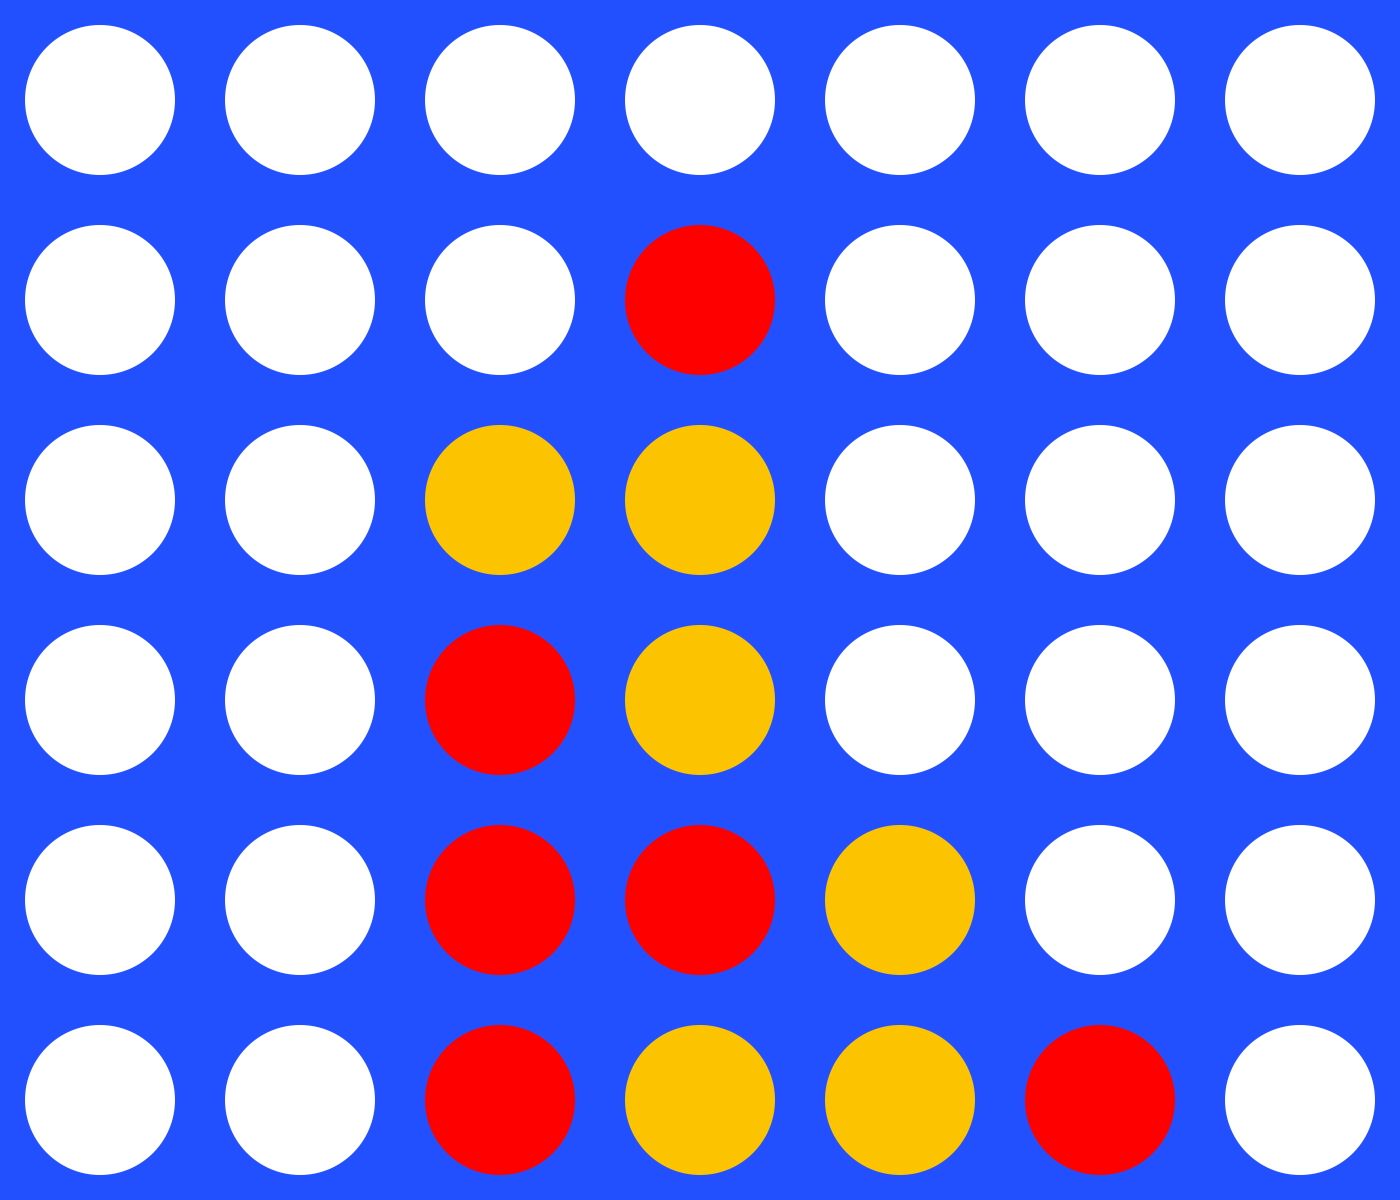
\includegraphics[width=0.5\textwidth]{connectFourExample}
\captionof{figure}{elo rating win probability for \(r_b = 0\)}
\label{fig:connect4ImageOne}
\end{center}

If red is the current player than:
\[
X = \left[
\begin{matrix}
\mathColor{black}{0} & \mathColor{black}{0} & \mathColor{black}{0} & \mathColor{black}{0} & \mathColor{black}{0} & \mathColor{black}{0} & \mathColor{black}{0}\\
\mathColor{black}{0} & \mathColor{black}{0} & \mathColor{black}{0} & \mathColor{red}{1}     & \mathColor{black}{0} & \mathColor{black}{0} & \mathColor{black}{0}\\
\mathColor{black}{0} & \mathColor{black}{0} & \mathColor{\gold}{0} & \mathColor{\gold}{0} & \mathColor{black}{0} & \mathColor{black}{0} & \mathColor{black}{0}\\
\mathColor{black}{0} & \mathColor{black}{0} & \mathColor{red}{1}     & \mathColor{\gold}{0} & \mathColor{black}{0} & \mathColor{black}{0} & \mathColor{black}{0}\\
\mathColor{black}{0} & \mathColor{black}{0} & \mathColor{red}{1}     & \mathColor{red}{1}     & \mathColor{\gold}{0} & \mathColor{black}{0} & \mathColor{black}{0}\\
\mathColor{black}{0} & \mathColor{black}{0} & \mathColor{red}{1}     & \mathColor{\gold}{0} & \mathColor{\gold}{0} & \mathColor{red}{1}     & \mathColor{black}{0}\\
\end{matrix}
\right]
\]\[
Y= \left[
\begin{matrix}
\mathColor{black}{0} & \mathColor{black}{0} & \mathColor{black}{0} & \mathColor{black}{0} & \mathColor{black}{0} & \mathColor{black}{0} & \mathColor{black}{0}\\
\mathColor{black}{0} & \mathColor{black}{0} & \mathColor{black}{0} & \mathColor{red}{0}     & \mathColor{black}{0} & \mathColor{black}{0} & \mathColor{black}{0}\\
\mathColor{black}{0} & \mathColor{black}{0} & \mathColor{\gold}{1} & \mathColor{\gold}{1} & \mathColor{black}{0} & \mathColor{black}{0} & \mathColor{black}{0}\\
\mathColor{black}{0} & \mathColor{black}{0} & \mathColor{red}{0}     & \mathColor{\gold}{1} & \mathColor{black}{0} & \mathColor{black}{0} & \mathColor{black}{0}\\
\mathColor{black}{0} & \mathColor{black}{0} & \mathColor{red}{0}     & \mathColor{red}{0}     & \mathColor{\gold}{1} & \mathColor{black}{0} & \mathColor{black}{0}\\
\mathColor{black}{0} & \mathColor{black}{0} & \mathColor{red}{0}     & \mathColor{\gold}{1} & \mathColor{\gold}{1} & \mathColor{red}{0}     & \mathColor{black}{0}\\
\end{matrix}
\right]
\] For clarification the numbers are colored in the same color as the stones at that position. After reanrangind dimensions \(i_n\) is:
\[
i_n = \left[
\begin{matrix}
\mathColor{black}{[0,0]} & \mathColor{black}{[0,0]} & \mathColor{black}{[0,0]} & \mathColor{black}{[0,0]} & \mathColor{black}{[0,0]} & \mathColor{black}{[0,0]} & \mathColor{black}{[0,0]}\\
\mathColor{black}{[0,0]} & \mathColor{black}{[0,0]} & \mathColor{black}{[0,0]} & \mathColor{red}{[1,0]}     & \mathColor{black}{[0,0]} & \mathColor{black}{[0,0]} & \mathColor{black}{[0,0]}\\
\mathColor{black}{[0,0]} & \mathColor{black}{[0,0]} & \mathColor{\gold}{[0,1]} & \mathColor{\gold}{[0,1]} & \mathColor{black}{[0,0]} & \mathColor{black}{[0,0]} & \mathColor{black}{[0,0]}\\
\mathColor{black}{[0,0]} & \mathColor{black}{[0,0]} & \mathColor{red}{[1,0]}     & \mathColor{\gold}{[0,1]} & \mathColor{black}{[0,0]} & \mathColor{black}{[0,0]} & \mathColor{black}{[0,0]}\\
\mathColor{black}{[0,0]} & \mathColor{black}{[0,0]} & \mathColor{red}{[1,0]}     & \mathColor{red}{[1,0]}     & \mathColor{\gold}{[0,1]} & \mathColor{black}{[0,0]} & \mathColor{black}{[0,0]}\\
\mathColor{black}{[0,0]} & \mathColor{black}{[0,0]} & \mathColor{red}{[1,0]}     & \mathColor{\gold}{[0,1]} & \mathColor{\gold}{[0,1]} & \mathColor{red}{[1,0]}     & \mathColor{black}{[0,0]}\\
\end{matrix}
\right]
\]
\paragraph{Neural Network Architecture} 
The neural network used by Alpha Zero consists of three main sub-modules, namely the residual tower, value head and policy head. The residual tower's purpose is to preprocess the data for the two heads. The value head determines the value \(v\) from the output of the residual tower. While the policy head computes the policy \(p\). The residual tower consists of a convolutional block followed by six residual blocks.\\
The convolutional block consists of the following: 
\begin{enumerate}
\item A convolutional layer consisting of 75 filters with a kernel size of 3 x 3
\item Batch normalization \cite{ioffe2015batch}
\item A non-linear rectifier (LeakyReLU).
\end{enumerate}
Every residual block consists of the following Modules:
\begin{enumerate}
\item A convolutional layer consisting of 75 filters with a kernel size of 3 x 3
\item Batch normalization \cite{ioffe2015batch}
\item A non-linear rectifier (LeakyReLU)
\item A convolutional layer consisting of 75 filters with a kernel size of 3 x 3
\item Batch normalization \cite{ioffe2015batch}
\item Batch normalization outputs are added to the block's input.
\item A non-linear rectifier (LeakyReLU)
\end{enumerate}
Outputs are then passed to the value and policy head of the network for further evaluation.
The value head consists of the following modules:
\begin{enumerate}
\item A convolutional layer consisting of 10 filters with a kernel size of 1 x 1
\item A fully connected layer of size 210
\item A non-linear rectifier (LeakyReLU)
\item A fully connected layer of size 1
\item \(tanh\) activation function
\end{enumerate}
The policy head consists of the following modules:
\begin{enumerate}
\item A convolutional layer consisting of 2 filters with a kernel size of 1 x 1
\item A fully connected layer of size 1
\end{enumerate}
The output of the policy head \(p_{pre}\) is then masked with the allowed actions in such a way that \(p_{pre}\) is \(-1000\) for all non-allowed actions. Finaly \(p_{pre}\) is than passed thought the softmax function to form \(p\):
\begin{equation}\label{eq:nn:policyDefinition}
p = \text{softmax}(p_{pre})
\end{equation}

\paragraph{Training}\label{sec:Methods:NN:A0:Training}
Training is performed in batches of \(256\) states. The value head is updated using mean square error, the policy head is updated using mean square error as well but all non-legal action predictions are assumed to have been correct, to avoid unnecessary updating of the neural network. The value, the neural network is trained to predict for a certain MCTS node \(n\), is equivalent to 1 if the player who took an action at node \(n\) won, \(-1\) if that player lost and \(0\) if the game ended in a tie. The policy \(p_{y_{a_l}}\) to train for, for a given legal action \(a_l \in \mathbb A(n)\) is:
\begin{equation} \label{eq:NN:policy_computation}
p_{y_{a_l}} = \frac{N(n, a_l)}{\sum_{a\in \mathbb A(n)} N(n, a)}
\end{equation}
For non legal actions \(a_n \in (\mathbb A - \mathbb A(n))\), \(p_{y_{a_n}}\) is defined as:
\begin{equation} \label{eq:NN:policy_computation_nonlegal}
p_{y_{a_n}} = p_{x_{a_n}} 
\end{equation}
where \(p_x\) is the predicted policy.


\subsection{Data generation}
The data used to train the neural network is generated by letting the best agent play several games against itself, until enough data has been generated to allow for training. In every game, at every game state, the MCTS performs 50 simulations. Once the simulations are done the action is chosen.
\subsubsection{Action selection}\label{sec:training:actionSelection}
There are two methods for action selection for a given node \(n_t\): deterministic and probabilistic. The former will always return the action \(a = argmax(N(\mathcal{E}(n_t, a \in \mathbb A(n_t))))\) of the most traversed edge, while the latter will return a random action where the probability of selecting an action \(a_i \in A(n_t)\) is:
\begin{equation} \label{eq:ActionSelection:Probabilistic}
P(X=a_i, n_t) = \frac{N(\mathcal{E}(n_t, a_i))}{\sum_{j \in \mathbb A(n_t)} N(\mathcal{E}(n_t, j))}
\end{equation}
(\(A(s)\) are the allowed actions for state \(s\).) To determine the action selection method a constant 'probabilitic\_moves' is defined. The selection is probabilitic if \(t < \text{probabilistic\_moves}\) and deterministic if not.

\subsubsection{Memory}
\label{sec:memory}
The memory stores a certain amount of game states \(g \in \mathbb G\), its action values \(v \in \mathbb R^{|\mathbb A|}\) and the true reward \(r \in \mathbb \{1, -1, 0\}\). Togather they make up a memroy element. The memory stores memory elements in a long list \(\iota\). After an action has bean selected, but befor any updates to the game simulation are made, the current game state is passed to temporary memory allong with its action values \(v\). Togather they create a new memory element. This elements \(r\) is currently undefined. \(v\) is defined as: 
\begin{equation} \label{eq:Memory:ActionValuesDefinition}
v_a = 
\begin{cases}
P(X=a, \mathcal N(g)) & a \in \mathbb A(g)\\
p_a &
\end{cases}
\end{equation}
\(p\) is defined in \equationref{eq:nn:policyDefinition}, and \(P\) is defined in \equationref{eq:ActionSelection:Probabilistic}

\paragraph{Memory update}
Once the game is done, the winning player is determined and a value \(v_m\) assigned to every state in the temporary memory. \(v_m\) is 1 if the player taking an action at that state won, -1 if he lost and 0 if the game ended in a draw. The updated states are then passed to memory.

\paragraph{Model Training}
Once the memory size exceeds 30'000 states, the self-playing stops and the neural network is trained as described in section:  \ref{sec:Methods:NN:A0:Training}.

\subsection{Model evaluation}
In order to train the neural network a best player generates data used to train the current network.
After every time the current neural network has bean updated it plays 20 games against the best player. If it wins more than \(1.3\) times as often as the current best agent, it is considered better, the current neural network is saved to file and the current best neural network is replaced with the current one. It is advantageous to force the network to score \(1.3\) times better as it reduces the chance of the network just getting lucky. For example in the following tournament betwean the current player and best player.
\\
\begin{center}\begin{tabular}{|c|c|c|}
\hline
gameId & current reward & best reward\\\hline
1 & 1 & -1\\
0 & 0 & 0 \\
2 & -1& 1 \\
3 & 1 & -1\\\hline
wins & 2 & 1 \\\hline
\end{tabular}\end{center}
Because \(1 \cdot 1.3 > 2\) the current player beat the best one and therefor the best will be replaced by the current one and the current is saved to file.

\section{Evaluation}
To give us an idea of how good a player is, it would be useful to express performance using a single number. This number should not only give us a ranking but also allow for predictions of the winner of a game between two agents and thus give us a measure of the relative strength of the agent. One such rating method is the elo-rating method. \cite{elo1978rating}
\subsection{Elo-rating} \label{sec:Evaluation:elo-rating}
The elo-rating system assigns every player \(p\) a number \(r_p \in \mathbb{R}^+\). Negative numbers are technically allowed but discouraged furthermore \(r_p \in  \mathbb N\) is encouraged. In general, the larger \(r_p\) the better the player. More specifically: given two players \(a\) and \(b\) with elo ratings \(r_a\) and \(r_b\) the expected chance \(E\) of \(a\) winning against \(b\) is\cite{silver2018general}:
\begin{equation} \label{eq:elo_pred}
E = \frac{1}{1 + e^{(r_b-r_a)/400}}
\end{equation}
\begin{center}
\includesvg[width=0.8\columnwidth]{images/elo}
\captionof{figure}{elo rating win probability for \(r_b = 0\)}
\end{center}
This function describes a sigmoid curve which makes sense, because if the players have major strength discrepancies \(E\) converges to \(1\) or \(0\). When \(a\) and \(b\) play a game against each other their elo ratings are updated as follows\cite{elo1978rating}:

\begin{equation} \label{eq:elo_update}
r_{n+1} = r_n + K(W - E)
\end{equation}
with:
\begin{description}
\item \(r_{n+1}\) the new rating for the player.
\item \(r_{n}\) the current rating of the player.
\item \(W = s_a\) is defined by equation \ref{eq:elo_score} where \(a\) is the player to be updated.
\item \(E\) the expected chance of winning, see equation \ref{eq:elo_pred}.
\item \(K\) is a constant controlling the sensitivity of the update function.
\end{description}
However, to avoid slow convergence of elo-ratings a more direct formula is used to approximate the rating of an agent \(a\). This is done by playing a predetermined amount of games against player \(b\) whose elo-rating is known and unchanged throughout this process. First, \(a\) and \(b\) play a predetermined amount of games \(m\) and the score \(s_a\) of \(a\) is computed as:
\begin{equation} \label{eq:elo_score}
s_a = \frac{1}{m}\sum\left\{
\begin{array}{ll}
1 &              a\textrm{ wins} \\
\frac{1}{2} & \textrm{tie}\\
0 &              a\textrm{ looses}\\
\end{array}
\right.
\end{equation}
Assuming that this is the probability of \(a\) winning against \(b\), \(a\)'s elo rating can be computed by solving equation \ref{eq:elo_pred} to \(r_a\):
\begin{equation} \label{eq:elo_back}
r_a = r_b - ln\left(\frac{1-s_a}{s_a}\right) \cdot 400
\end{equation}
\begin{center}
\includesvg[width=0.8\columnwidth]{images/elo_back}
\captionof{figure}{elo inverse function}
\end{center}
Since a ranking of the agents already exists, i.e. the version of the agent, because every version has to be able to beat the previous one. Therefore, an agent's elo-rating can be computed by playingy against an older version and then using equations \ref{eq:elo_score} and \ref{eq:elo_back} to determine its elo rating. 
\subsection{elo implementation}
The elo-rating of all agents is handled by a secondary server that is currently running on my backup computer. This server stores the elo values computed by the AI server. The Elo server stores an identity value for every agent. This value is the AI version for the AI and a negative number for human players. The system can request the elo rating of a certain player, set a player's elo rating, update the elo rating of a player and give new clients a unique key which unfortunately does not work for IOS clients. The computer's elo-ratings are predetermined and fixed. They are computed by having each player play against the previous player and using equation \ref{eq:elo_back} to set their elo-rating. Human players have a starting rating. They then play the agent with the closest rating to their own or they can request a specific version (except on IOS where the player will always play the best version). After every game, the player's rating is adjusted in accordance with equation \ref{eq:elo_update}.
\subsubsection{Relativity of the Elo-rating}
The only major problem is that elo is a relative rating. The rating of any other agent depends on its performance against other agents and their elo-rating. Therefore, one must give the system a base rating for a certain agent. In this case, there are no previously known elo-rated agents, so, the untrained agent is defined to have an elo rating of 100. All other elo ratings are relative to that.

\subsection{Elo results}
\begin{center}
	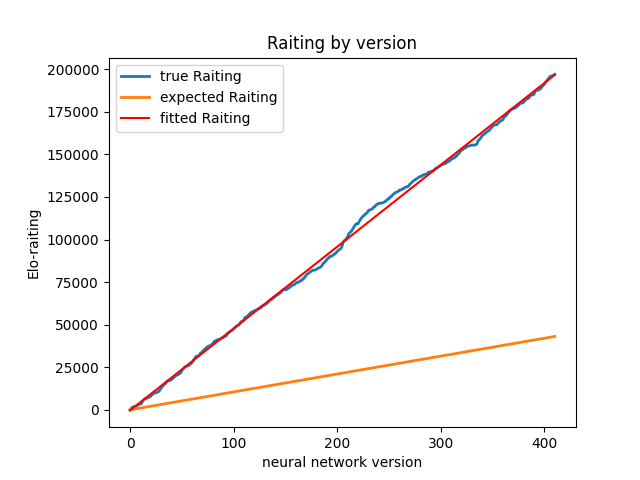
\includegraphics[width=0.9\textwidth]{eloRaitingByVersion}
	\captionsetup{width=.8\linewidth}
	\captionof{figure}{Elo ratiging of agents based on there version along with the expected minimal raiting and the best fitting raiting.}
	\label{img:eloByVersion}
\end{center}
The expected raiting \(E(a)\) of any agent version \(a\) must in genrall be greater than the raiting of the last version \(E(a) > E(a-1)\). Furthermore the expected minimal increas in raiting \(\Delta E\) is:
\begin{equation}
\Delta E = -ln(\frac{1-s_a}{s_a})\cdot 400
\end{equation}
As a certain scoring threashold \(\theta\) was used during training to minimize the effect of noise in the evaluation. A prediction of \(s_a\) can be made. Given that \(s_a\) and \(s_b\) are the scores of two players that play aginst each other than by definition
\begin{equation}
s_a + s_b = 1
\end{equation}
Due to the emposed scoring threshold \(\theta\) and the assumption that there are no ties:
\begin{equation}
s_a \geqslant s_b \cdot \theta
\end{equation}
For \(\theta = 1.3\) this means that:
\begin{equation}
\Delta E \geqslant -ln\left(\frac{1}{\theta}\right)\cdot 400 \cong 105
\end{equation}
Collected data shows this to be true \imgRef{img:eloByVersion} the same data shows that the average \(\Delta E \cong \FittedEloRaiting\) which would equate to a \(\theta\) of .

\begin{equation}
\Delta E = \frac{1}{e^{\frac{-\Delta E}{400}}} \cong \FittedEloRaiting
\end{equation}
This raiting would converge to infinity however the time to find a better strategy would limit this. One would expect that as the mount of training steps encrieses the agents learning would slow but still converge to optimal play. This has been shown in Go chess and Shogi this version shows this behaviour to some extend. However its not as obvious as with go and Shogi. This is mostly due to the asynchronous training method.

\section{Server and Clients}
In computer science Server Client communications are a form of distributed application, that allows multiple machines to communicate and share data. In general the server will wait for connections, the client will initialize a connection with a server. To accomplisch this, the server must listen to a certain port and the client must know the servers ip. In our case the cummunications use the TCP and HTTP protocols. Alpha Zero uses three distict servers: an AI server, a data server and a appache web server. The simplest is the web server.
\subsection{Web Server}
Alpha Zero's web server uses the appache webserver application. The webserver is used to host static files such as the source code for the IOS client, a debug version of the same client, the demain name of the ai server and the domain name of the data server. All these files are located at \href{http://wandhoven.ddns.net/code/AlphaZero/}{http://wandhoven.ddns.net/code/AlphaZero/}
\subsubsection{Domain Name}
A domain name is a way to avoid refering to servers by ip addres. Using ip addresses is problematic in multiple ways. Such as the fact that ip's can change over time or that humans have trouble understanding and memorizing lists of numbers for instance on the 1.Mär.2021 the IPv6 of \textbf{google.com} resolved to 2a00:1450:400a:803::200e. No human would understand this implicitly. 

\subsection{Data Server}
The data server stores all global information which was just the rating to begin with but was later expanded to handle all data. This explains the somewhat strange comunication protocol. Requests to the server begin by sending a 4 byte signed intager \(a\) identifying the general action the server must perform. The first action \(a=1\) will return the elo rating of a certain agent.
This will require a further 4 bytes identifying the agent. The second action \(a=2\) will set an agents elo rating. Two 4 byte intagers are sent the first identifying the agent and the second the elo rating to set to. The Third action \(a=-1\) will require a 4 byte signed intager\(e\) and return the agents identifier with an elo rating equal to \(r\) defined as:
\begin{equation}
r = min(\left\{x \in\mathbb E | x \leq e \right\})
\end{equation}
where \(\mathbb E\) is the set of the elo ratings of all agents. The last action \(a=-2\) will access the custom data part of the server. This subsection will require an intager describing how manny bytes the request consists of. The request is encripted using the python pickle library and consist of ether a tuple containing a string and a list os strings or a tuple containing a string a list of strings and any other data type. In the former case the system will return the value of the saved data asociated with that request. In the later case the value of the associated the variable will be set to what ever the third value is.
\subsubsection{Variable Association}
The first two variables sent being a string \(f\) and a list \(k\). \(f\) tells the server in whitch file the variable is being stored. Therefor the server will load the json file with the name saved in \(f\). \(k\) is the list of keys used to index the dictionary saved in \(f\). Should that key not exist an empty dict is added containing it except if it is the last in which case it would be ignored.

\subsection{AI Server}
The AI server is used to evaluate a state and determine the best action using Alpha Zero. This is done my sending the server the sate and waiting for it to send back the action.
\subsubsection{state transmition}
To send a state to the server the states \(6 \times 7\) board is converted into a 85 Boolean values. The first 42 Boolean represent weather or not the starting player has a stone at that position, positions are mapped from left to right and than top to bottom. The table below shows order in which the Positions will be added to the Boolean list. The next 42 Booleans are identical to the first but for the non-starting player. The last position tells the server which player is taking the next action.
\begin{center}
\begin{tabular}{| c | c | c | c | c | c | c |}
 \hline
0 & 1 & 2 & 3 & 4 & 5 & 6  \\\hline
7 & 8 & 9 & 10 & 11 & 12 & 13\\\hline
14 & 15 & 16 & 17 & 18 & 19 & 20 \\\hline
21 & 22 & 23& 24 & 25 & 26 & 27 \\\hline
28 & 29 & 30 & 31 & 32 & 33 & 34 \\\hline
35 & 36 & 37 & 38 & 39 & 40 & 41 \\\hline
\end{tabular}
\end{center}
The following game state \imgRef{fig:connectFourExample} at wich the starting player is at turn.
\begin{center}
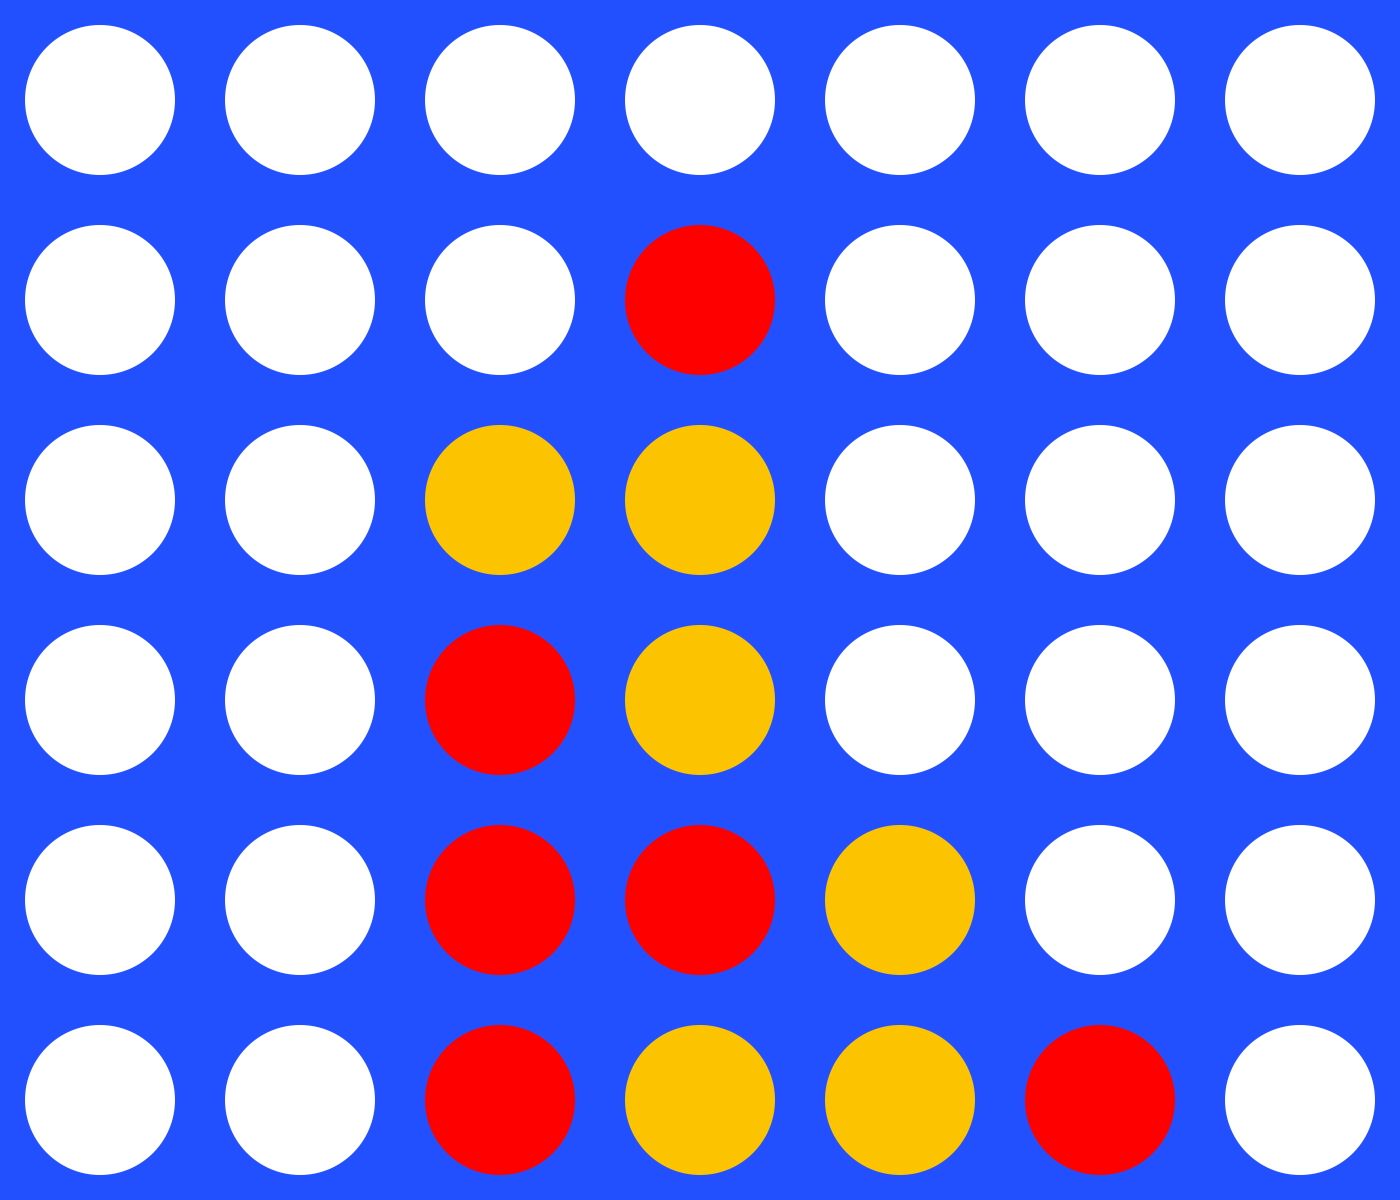
\includegraphics[width=0.5\textwidth]{connectFourExample}
\captionof{figure}{elo rating win probability for \(r_b = 0\)}
\label{fig:connectFourExample}
\end{center}
The state array \(a\) is:
\begin{equation}
a =
\text{vec}\left(\left[\begin{matrix}
\mathColor{black}{0} & \mathColor{black}{0} & \mathColor{black}{0} & \mathColor{black}{0} & \mathColor{black}{0} & \mathColor{black}{0} & \mathColor{black}{0}\\
\mathColor{black}{0} & \mathColor{black}{0} & \mathColor{black}{0} & \mathColor{red}{1}     & \mathColor{black}{0} & \mathColor{black}{0} & \mathColor{black}{0}\\
\mathColor{black}{0} & \mathColor{black}{0} & \mathColor{\gold}{0} & \mathColor{\gold}{0} & \mathColor{black}{0} & \mathColor{black}{0} & \mathColor{black}{0}\\
\mathColor{black}{0} & \mathColor{black}{0} & \mathColor{red}{1}     & \mathColor{\gold}{0} & \mathColor{black}{0} & \mathColor{black}{0} & \mathColor{black}{0}\\
\mathColor{black}{0} & \mathColor{black}{0} & \mathColor{red}{1}     & \mathColor{red}{1}     & \mathColor{\gold}{0} & \mathColor{black}{0} & \mathColor{black}{0}\\
\mathColor{black}{0} & \mathColor{black}{0} & \mathColor{red}{1}     & \mathColor{\gold}{0} & \mathColor{\gold}{0} & \mathColor{red}{1}     & \mathColor{black}{0}\\
\end{matrix}
\right]\right)
\frown vec
\left(\left[
\begin{matrix}
\mathColor{black}{0} & \mathColor{black}{0} & \mathColor{black}{0} & \mathColor{black}{0} & \mathColor{black}{0} & \mathColor{black}{0} & \mathColor{black}{0}\\
\mathColor{black}{0} & \mathColor{black}{0} & \mathColor{black}{0} & \mathColor{red}{0}     & \mathColor{black}{0} & \mathColor{black}{0} & \mathColor{black}{0}\\
\mathColor{black}{0} & \mathColor{black}{0} & \mathColor{\gold}{1} & \mathColor{\gold}{1} & \mathColor{black}{0} & \mathColor{black}{0} & \mathColor{black}{0}\\
\mathColor{black}{0} & \mathColor{black}{0} & \mathColor{red}{0}     & \mathColor{\gold}{1} & \mathColor{black}{0} & \mathColor{black}{0} & \mathColor{black}{0}\\
\mathColor{black}{0} & \mathColor{black}{0} & \mathColor{red}{0}     & \mathColor{red}{0}     & \mathColor{\gold}{1} & \mathColor{black}{0} & \mathColor{black}{0}\\
\mathColor{black}{0} & \mathColor{black}{0} & \mathColor{red}{0}     & \mathColor{\gold}{1} & \mathColor{\gold}{1} & \mathColor{red}{0}     & \mathColor{black}{0}\\
%&&& 1 &&&]\\
\end{matrix}\right]\right)\frown \left<1\right>
\end{equation}




\subsubsection{action selection}
The AI's action is selected by running MCTS simulations and choosing the action with the most evaluations. It is the same algorythem as the deterministic method in training defined in \sectionref{sec:training:actionSelection}.
\subsubsection{action transition}
The action is stored as a 4 byte integer which is just transmitted using its binary representation.

\section{Further definitions}
\subsection{Hadamard product}\label{sec:hadamerd_product}
Let \(A\) and \(B\) be 2 \(m \times n\) matrices. For all \(i \in [1, m]\) and \(j \in [1, n]\)
the hadamard product \(A \circ B\) is defined as:
\begin{equation} \label{eq:defs:Hadamard product}
\left(A \circ B\right)_{ij} = A_{ij} \cdot B_{ij}
\end{equation}
For example consider the following \(2 \times 3\) matrix's:
\[
\left[
\begin{array}{ll}
a_{11} & a_{12} \\
a_{21} & a_{22} \\
a_{31} & b_{32} \\
\end{array}
\right] \circ 
\left[
\begin{array}{ll}
b_{11} & b_{12} \\
b_{21} & b_{22} \\
b_{31} & b_{32} \\
\end{array}
\right] = 
\left[
\begin{array}{ll}
a_{11}b_{11} & a_{12}b_{12} \\
a_{21}b_{21} & a_{22}b_{22} \\
a_{31}b_{31} & a_{32}b_{32} \\
\end{array}
\right]
\]

\subsection{Inner Product}
\subsubsection{Matrixes}
Let \(A\in \mathbb{R}^{m \times n}\) and \(B\in \mathbb{R}^{m \times n}\) be two \(n \times m\) matrices. \\Let their Inner product \(\left<A, B\right>_I:\; \mathbb{R}^{m \times n},~\mathbb{R}^{m \times n} \to \mathbb{R}\) be defined as:
\begin{equation} \label{eq:defs:Inner_product}
\left<A, B\right>_I = \sum_{i=1}^{m}\sum_{j=1}^{n} A_{ij}B_{ij} = \sum_{i=1}^{m}\sum_{j=1}^{n} (A \circ B)_{ij}
\end{equation}
For example consider the following \(2 \times 3\) matrices:
\[
\left<
\begin{bmatrix}
a_{11} & a_{12} \\
a_{21} & a_{22} \\
a_{31} & b_{32} \\
\end{bmatrix}
\begin{matrix} \\\\,\end{matrix}~
\begin{bmatrix}
b_{11} & b_{12} \\
b_{21} & b_{22} \\
b_{31} & b_{32} \\
\end{bmatrix}\right>_I
= \;
\begin{array}{ll}
     a_{11}b_{11} + a_{12}b_{12} + a_{21}b_{21}\\
+~a_{22}b_{22} + a_{31}b_{31} + a_{32}b_{32} 
\end{array}
\]

\subsubsection{3D Tensors}
Let \(A \in \mathbb{R}^{m \times n \times d}\) and \(B \in \mathbb{R}^{m \times n \times d}\) be two \(m \times n \times d\) tensors.\\
Let the Inner product \(\left<A, B\right>_I : \mathbb{R}^{m \times n \times d}, \mathbb{R}^{m \times n \times d} \to \mathbb{R}\) be defined as:
\begin{equation}\label{eq:defs:Inner_product_3d}
\left<A, B\right>_I = \sum_{i=0}^{m} \left<A_{i}, B_{i}\right>_I
\end{equation}

\begin{sidewaysfigure}[ht]
    \centering
	\captionsetup{width=.9\linewidth}
    \includesvg[width=\columnwidth]{images/MCTS-steps.svg}
		\caption[width=0.7\columnwidth]{MCTS simulation steps. In this diagram the numbers in the node represents \(Q\) and the number on the arrow is \(P\). The red nodes are leaf nodes and the green one is the leaf node \(n_L\). During the \textbf{selection} phase \(\sigma\) is used to find succesive nodes until the node \(n_L\) is reached. This is shown with the arrows. During the \textbf{expansion} phase new nodes and edges are added for all possible actions at the node \(n_L\). The \textbf{evaluation} phase gives the new nodes the following values \(Q = 0\) and \(P = \pi_a\). The value of the leaf \(V\) is than used during the \textbf{backfill} phase to update the \(Q\)'s of all nodes traversed during selection.}
		\source{modified from \url{https://en.wikipedia.org/wiki/File:MCTS-steps.svg}\\File available under \href{https://creativecommons.org/licenses/by-sa/4.0/deed.en}{Creative Commons Attribution-Share Alike 4.0 International} at \url{http://wandhoven.ddns.net/edu/AlphaZero/AlphaZeroTheory/images/MCTS-steps.svg}}
	\label{MCTS-simulation}
\end{sidewaysfigure}

\subsection{Submatrix}
\label{sec:Ref:submatrix}
Let \(m = m_{ijk}\) be an \(m\times n\times o\) dimesional tensor.\\
Let \(Q_1 \subseteq [1,m ]\) , \(Q_2 \subseteq [1, n]\) and \(Q_3 \subseteq [1,o]\).\\
The subtensor \(m[Q_1, Q_2, Q_3]\) consists of all  \(m_{i'j'k'}\) where \( i' \in Q_1\), \( j' \in Q_2\) and \( k' \in Q_3\).\\
\(m[Q_1, Q_2, Q_3]\) is a \(|Q_1| \times |Q_2| \times |Q_3|\) tensor.\\
%see \href{https://planetmath.org/submatrixnotation}{https://planetmath.org/submatrixnotation} matrix definition.

\subsection{Binary Cross Entropy}
Let \(N \in \mathbb{N}^+\) be the amount of values in the batch.\\
Let \(x  \in \mathbb{R}^N\) be the models prediton for a given input.  \(s\)\\
Let \(y  \in \mathbb{R}^N\) be the labels for the input \(s\).\\
Let \(\beta(x, y)\) be the Binary Cross Entropy loss function.
\[
\beta(x, y) = -\frac{1}{N}\sum_{i=0}^{N}y_i\cdot log(x_i) + (1 - y_i) \cdot log(1 - x_i)
\]

\subsection{Vectorization}  \label{sec:ref:vectorization}
The vectorization of a \(m \times n\) matrix \(A\), denoted \(\text{vec}(A)\), is the \(mn \times 1\) column vector obtained by stacking the columns of the matrix A on top of one another: 
\begin{equation}\label{eq:ref:vectorization}
\text{vec}(A) = \left[
A_{11}\,\dots\,A_{1m}\,A_{21}\,\dots \,A{2m}\,\dots\,A_{n1}\,\dots\,A{nm}
\right]^T
\end{equation}

cited verbatim from:\cite{vectorization_2021}\\
For example the \(3\times 2\) matrix \(A=\left[
\begin{matrix}
a & b & c\\
d & e & f\\
\end{matrix}
\right]\), vectorizes to:
\[
\text{vec}(A) = \left(
\begin{matrix}
a\\
b\\
c\\
d\\
e\\
f\\
\end{matrix}
\right)
\]
\subsection{Vector Concatination}
Vector Concatination of two vectors \(v\) and \(u\) of dimensions \(n_v\) and  \(n_u\), denoted \(v\frown u\), is the \(n_v + n_u\) dimensional vector optained by placing both vectors one behind the other.
\begin{equation} \label{eq:ref:vecConcatination}
v\frown u = \left(
\begin{matrix}
v_1\\
\vdots\\
v_{n_v}\\
u_1\\
\vdots\\
u_{n_u}\\
\end{matrix}
\right)
\end{equation}

\bibliographystyle{plain}
\bibliography{bibliography}

\section*{Acknowledgements}
\begin{itemize}
\item Leonie Scheck, Frederik Ott, Nico Steiner, Wolfgang Wandhoven for aiding in evaluating the AI aginst human players and providing playbacks.
\item Chrisopher Nitch for pressing space once.
\end{itemize}
\end{document}
